\newpage

\subsection{Introduction to Object Oriented Programming}

Object-oriented programming (OOP) is a programming paradigm using "objects" – usually instances of a class – consisting of data fields 		and methods together with their interactions – to design applications and computer programs. Programming techniques may include 		features such as data abstraction, encapsulation, messaging, modularity, polymorphism, and inheritance. Many modern programming 		languages now support forms of OOP, at least as an option.\\

An object-oriented program may be viewed as a collection of interacting objects, as opposed to the conventional model, in which a program is seen as a list of tasks (subroutines) to perform. In OOP, each object is capable of receiving messages, processing data, and sending messages to other objects. Each object can be viewed as an independent "machine" with a distinct role or responsibility. The actions (or "methods") on these objects are closely associated with the object. For example, OOP data structures tend to "carry their own operators around with them".\\

The terms "objects" and "oriented" in something like the modern sense of object-oriented programming seem to make their first appearance at MIT in the late 1950s and early 1960s. 
    \subsubsection{Features of OOPs}
    \begin{itemize}
    \item OPPs abbreviated as an Object Oriented Programming Language.
    \item Object Oriented Programming (OOP) is a Programming methodology that uses ‘object’ to design applications and computer programs.
	\item Object-Oriented Programming (OOP) is a software development paradigm that suggests developers to split a program in building blocks known as objects. The OOP paradigm allows developers to define the object's data,functions, and its relationship with other objects.
	\item It utilizes various techniques from previously established paradigms including Inheritance, Polymorphism and Encapsulation.
	\item The ability to define a class and create instances of classes is one of the most important capabilities of any Object Oriented Programming.
	\end{itemize}
	\subsubsection{Object}
	\begin{itemize}
	\item In everyday life, an object is anything that is identifiably a single material item i.e. a Car, a book, a document etc.
	\item In technical language Object is called as a instance of class.
	\item Objects are key understanding of Object oriented programming.
	\item In other words, break each program into lots of units and design each unit to perform a clearly specified role within the pro
	\end{itemize}
	\subsubsection{Class}
	\begin{itemize}
	\item A Class is a Blueprint from which individual objects are created.
	\item In OOP you program a class as a template for a specific object or groups of objects that will always have the same features.
	\end{itemize}
	\subsubsection{Encapsulation}
	Encapsulation is an Object Oriented Programming concept that binds together the data and functions that manipulate the data, and that keeps both safe from outside interference and misuse. Data encapsulation led to the important OOP concept of data hiding.
Data encapsulation is a mechanism of bundling the data, and the functions that use them and data abstraction is a mechanism of exposing only the interfaces and hiding the implementation details from the user.\\
Neither too much access nor too much control must be placed on the operations in order to make the class user friendly. Hiding the implementation details and providing restrictive access leads to the concept of abstract data type. Encapsulation leads to the concept of data hiding.[3]

	\subsubsection{Inheritance}
	In object-oriented programming (OOP), inheritance is a way to reuse code of existing objects, or to establish a subtype from an existing object, or both, depending upon programming language support. In classical inheritance where objects are defined by classes, classes can inherit attributes and behavior from pre-existing classes called base classes, super classes, parent classes or ancestor classes. The resulting classes are known as derived classes, subclasses or child classes. The relationships of classes through inheritance gives rise to a hierarchy. In prototype-based programming, objects can be defined directly from other objects without the need to define any classes, in which case this feature is called differential inheritance. The figure1 shows the inheritance as:
%\image{1.2}{images/image.png}{Inheritance Example}
	\begin{figure}[h]
	\centering
	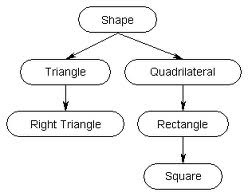
\includegraphics[scale=0.7]{images/image.jpg}
	%
\includegraphics[scale=0.13]{gne.png}
	\caption{Inheritance example}
	\end{figure}
	
	\subsubsection{Data Hiding}
	\begin{itemize}
	\item Data Hiding is also known as Encapsulation.
	\item Encapsulation is the process of combining data and function into a single unit called class.
	\item Data Hiding is the mechanism where the details of the class are hidden from the user.
	\item The user can perform only a restricted set of operations in the hidden member of the class.
	\item Encapsulation is a powerful feature that leads to information hiding,abstract data type and friend function.
	\item They encapsulate all the essential properties of the object that are to be created.
	\item Using the method of encapsulation the programmer cannot directly access the class.
	\end{itemize}
	It provides the following features:
	\begin{itemize}
	\item The advantage of data encapsulation comes when the implementation of the class changes but the interface remains the same.
	\item It is used to reduce the human errors. The data and function are bundled inside the class that take total control of maintenance 			and thus human errors are reduced. 
	\item Makes maintenance of application easier. 
	\item Improves the understandability of the application. 
	\item Enhanced Security.
	\end{itemize}

%\newpage

\subsection{Introduction to C++}
	C++ (pronounced "see plus plus") is a statically typed, free-form, multi-paradigm, compiled, general-purpose programming language. It is regarded as an intermediate-level language, as it comprises a combination of both high-level and low-level language features. Developed by Bjarne Stroustrup starting in 1979 at Bell Labs, it adds object oriented features, such as classes, and other enhancements to the C programming language. Originally named C with Classes, the language was renamed C++ in 1983,as a pun involving the increment operator.\newline
	C++ is one of the most popular programming languages and is implemented on a wide variety of hardware and operating system platforms. As an efficient compiler to native code, its application domains include systems software, application software, device drivers, embedded software, high-performance server and client applications, and entertainment software such as video games.Several groups provide both free and proprietary C++ compiler software.\\
C++ is the multi paradigm, compile, free form , general purpose, statistically typed programming language. This is known as middle 		level language as it comprises of low level and high level language features.
And there are some other things and advantages of this language over the C. This language of invented by Bjarne Stroustrup was working 	on the “C with classes” as his Ph.D.  topic. The first commercial implementation of the C++ was released in 1985 and before that the 		name of language was changed to “C++”. And some new features were added to the language and The main features of the C++ are
\begin{itemize}
\item Classes
\item Inheritance
\item Data abstraction and encapsulation
\item Polymorphism
\item Dynamic Binding
\item Message Passing
\end{itemize}
Here is a brief description of each features.
\begin{itemize}
\item {\bf{Classes:}}By using classes we can create user defined data types. In other words the class is the collection of set of data and code. The class allows us to do some things which are polymorphism, inheritance, abstraction, encapsulation which are our next features. The objects are the instances of classes.
The syntax for class is :
Class <class-name>
{   
//Body of class;
};
 \item{\bf{Inheritance:}}
 Inheritance allows one data type to acquire properties of other data types. Inheritance from a base class may be declared as public, protected, or private. If the access specifier is omitted, a “class” inherits privately, while a “struct” inherits publicly. This provides the idea of reusability that means we can add the new features to an existing class without modifying it.
 
 \item{\bf{Data Abstraction and Encapsulation:}}
  Encapsulation means hiding of data from the data structures or in other words wrapping up of data in single entity is known as Encapsulation. In this the data is not accessible to outside world and only the  functions are allowed to access it.  When we want to write the class in which we don’t have the knowledge about the arguments used to instantiate it then we can use templates in C++. Abstraction can be defined as the act of representing essential features without including background details.[5]
 
 \item{\bf{Polymorphism:}}
It means that the one interface can be used for many implementation so that object can behave differently for each implementation. The different types of polymorphism are static (Compile time) and dynamic (Run time).
 
 \item{\bf{Dynamic Binding:}}
It means that the linking of a procedure call to code to be executed in response to the call. A function call associated with a polymorphic reference depends on the dynamic type that reference. And at run-time the code matching the object under current reference will be called.
 \item{\bf{Message Passing:}}
  An object oriented program consists of the set of objects that communicate with each other. objects communicate with one another by sending and receiving information much the same way as people pass messages to one another. The concept of message passing makes it easier to direct model or simulate their real world counterparts.
	
\end{itemize}

\newpage

\subsection{MySQL Database Server}

{\bf MySQL}, the most popular Open Source SQL database management system, is
developed, distributed, and supported by Oracle Corporation. It is
based on the structure query language (SQL), which is used for adding,
removing, and modifying information in the database. Standard SQL
commands, such as ADD, DROP, INSERT, and UPDATE can be used with
MySQL.

MySQL can be used for a variety of applications, but is most commonly
found on Web servers. A website that uses MySQL may include Web pages
that access information from a database. These pages are often
referred to as "dynamic," meaning the content of each page is
generated from a database as the page loads. Websites that use dynamic
Web pages are often referred to as database-driven websites.

\begin{itemize}
\item {\bf MySQL is a database management system.}\\
A database is a structured collection of data. It may be anything from
a simple shopping list to a picture gallery or the vast amounts of
information in a corporate network. To add, access, and process data
stored in a computer database, you need a database management system
such as MySQL Server. Since computers are very good at handling large
amounts of data, database management systems play a central role in
computing, as standalone utilities, or as parts of other applications. 

\item {\bf MySQL databases are relational.}\\
A relational database stores data in separate tables rather than
putting all the data in one big storeroom. The database structures are
organized into physical files optimized for speed. The logical model,
with objects such as databases, tables, views, rows, and columns,
offers a flexible programming environment. You set up rules governing
the relationships between different data fields, such as one-to-one,
one-to-many, unique, required or optional, and “pointers” between
different tables.

\item {\bf MySQL software is Open Source.}\\
Open Source means that it is possible for anyone to use and modify the
software. Anybody can download the MySQL software from the Internet
and use it without paying anything. If you wish, you may study the
source code and change it to suit your needs. The MySQL software uses
the GPL (GNU General Public License).

\item {\bf The MySQL Database Server is very fast, reliable, scalable,
and easy to use.}\\
If that is what you are looking for, you should give it a try. MySQL
Server can run comfortably on a desktop or laptop, alongside your
other applications, web servers, and so on, requiring little or no
attention.

\end{itemize}

\newpage

\subsection{Apache Web Server}

Apache HTTP Server, commonly referred to as Apache (/pti/
-PA-chee), is a web server
software notable for playing a key role in the initial growth of the
World Wide Web. Apache is
developed and maintained by an open community of developers under the
auspices of the Apache
Software Foundation. The application is available for a wide variety
of operating systems, including
Unix, FreeBSD, Linux, Solaris, Novell NetWare, OS X, Microsoft
Windows, OS/2, TPF, and
eComStation. Released under the Apache License, Apache is open-source
software.\\
The goal of this project is to provide a secure, efficient and
extensible server that provides
HTTP services in sync with the current HTTP standards.

{\bf Following are main features of Apache Server:}

\begin{itemize}

\item Apache supports a variety of features, many implemented as compiled
modules which extend
the core functionality. These can range from server-side programming
language support
to authentication schemes. Some common language interfaces support
Perl, Python, Tcl,
and PHP. Popular authentication modules include mod access, mod auth,
mod digest,
and mod auth digest, the successor to mod digest. A sample of other
features include
Secure Sockets Layer and Transport Layer Security support ( mod ssl),
a proxy module
(mod proxy), a URL rewriter (mod rewrite), custom log files (mod log
config), and filtering
support (mod include and mod ext filter).
\item Apache features configurable error messages, DBMS-based
authentication databases, and
content negotiation. It is also supported by several graphical user
interfaces (GUIs).
\item It supports password authentication and digital certificate
authentication. Apache has a
built in search engine and an HTML authorizing tool and supports FTP.

\end{itemize}

\newpage

\subsection{GNU G++ Compiler}

The GNU Compiler Collection includes front ends for C, C++,
Objective-C, Fortran, Java, Ada, and Go, as well as libraries for
these languages (libstdc++, libgcj,...). GCC was originally written as
the compiler for the GNU operating system. The GNU system was
developed to be 100\% free software, free in the sense that it respects
the user's freedom.\\ \\
We strive to provide regular, high quality releases, which we want to
work well on a variety of native and cross targets (including
GNU/Linux), and encourage everyone to contribute changes or help
testing GCC. Our sources are readily and freely available via SVN and
weekly snapshots.\\ \\
Major decisions about GCC are made by the steering committee, guided
by the mission statement.\\ \\
You can invoke g++ on a source code file simply by typing

{\bf g++ filename}\\ \\
The default executable output of g++ is "a.out". It is also possible
to specify a name for the executable file at the command line by using
the syntax 

{\bf -o outputfile}\\ \\
, as shown in the following example: 

{\bf g++ filename -o outputfile}

\newpage
\subsection{Common Gateway Interface and C++}

The Common Gateway Interface, or CGI, is a set of standards that
define how information is exchanged between the web server and a
custom script.The CGI specs are currently maintained by the NCSA and
NCSA defines CGI is as follows:
\begin{itemize}
\item The Common Gateway Interface, or CGI, is a standard for external
gateway programs to interface with information servers such as HTTP
servers.
\item The current version is CGI/1.1 and CGI/1.2 is under progress.
\end{itemize}

\subsubsection{Web Browsing}

To understand the concept of CGI, let's see what happens when we click
a hyperlink to browse a particular web page or URL.

\begin{itemize}
\item Your browser contacts the HTTP web server and demand for the URL
ie. filename.
\item Web Server will parse the URL and will look for the filename. If
it finds requested file then web server sends that file back to the
browser otherwise sends an error message indicating that you have
requested a wrong file.
\item Web browser takes response from web server and displays either
the received file or error message based on the received response.
\end{itemize}

\subsubsection{CGI Architecture Diagram}

The following simple program shows a simple architecture of CGI:

%\image{0.7}{images/cgiarch.gif}{CGI Architecture Diagram}
	\begin{figure}[h!]
	\centering
	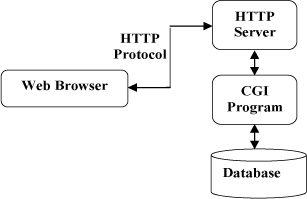
\includegraphics[scale=0.7]{images/cgiarch.png}
	%
\includegraphics[scale=0.13]{gne.png}
	\caption{CGI Architecture}
	\end{figure}

\newpage

\subsection{CGICC Library}

{\bf GNU CGICC } a C++ class library for writing CGI applications.

\subsubsection{Introduction to GNU Cgicc}

GNU cgicc is an ANSI C++ compliant class library that greatly
simplifies the creation of CGI applications for the World Wide Web.
cgicc performs the following functions:

\begin{itemize}

\item Parses both GET and POST form data transparently. 
\item Provides string, integer, floating-point and single- and
multiple-choice retrieval methods for form data. 
\item Provides methods for saving and restoring CGI environments to
aid in application debugging. 
\item Provides full on-the-fly HTML generation capabilities, with
support for cookies. 
\item Supports HTTP file upload. 

\end{itemize}

\subsubsection{Requirements}

GNU cgicc requires an ANSI-compliant C++ compiler supporting the C++
standard template library. cgicc is primarily developed on GNU/Linux
using gcc version 3.3, but it has been built using the following
compilers:

\begin{itemize}
\item gcc versions 2.8.1 and greater 
\item Hewlett-Packard aCC
\item Microsoft Visual C++ 6.0 
\end{itemize}

\newpage

\subsection{Make Utility}

{\bf make} - GNU make utility to maintain groups of programs.\\ \\
The purpose of the make utility is to determine automatically which
pieces of a large program need to be recompiled, and issue the
commands to recompile them. The manual describes the GNU
implementation of make, which was written by Richard Stallman and
Roland McGrath. Our examples show C programs, since they are most
common, but you can use make with any programming language whose
compiler can be run with a shell command. In fact, make is not limited
to programs. You can use it to describe any task where some files must
be updated automatically from others whenever the others change.\\ \\
To prepare to use make, you must write a file called the makefile that
describes the relationships among files in your program, and the
states the commands for updating each file. In a program, typically
the executable file is updated from object files, which are in turn
made by compiling source files.\\ \\
Once a suitable makefile exists, each time you change some source
files, this simple shell command: 

{\bf make} \\ \\
suffices to perform all necessary recompilations. The make program
uses the makefile data base and the last-modification times of the
files to decide which of the files need to be updated. For each of
those files, it issues the commands recorded in the data base. 

\newpage

\subsection{Boost Library}

Boost provides free peer-reviewed portable C++ source libraries.\\ \\
Boost libraries are intended to be widely useful, and usable across a
broad spectrum of applications. The Boost license encourages both
commercial and non-commercial use.\\ \\
Most of the Boost libraries are licensed under the Boost Software
License, designed to allow Boost to be used with both free and
proprietary software projects. Many of Boost's founders are on the C++
standards committee, and several Boost libraries have been accepted
for incorporation into both Technical Report 1 and the C++11 standard.

\newpage

\subsection{jwSMTP Library}

jwSMTP is a C++ library/code (GPL license) to facilitate sending email
programmatically. New in version 1.32.3 send mail in html format. All
you need worry about is who the mail is from, who to send it to and
the message itself, no network coding necessary. jwSMTP can send
attachments, send to multiple recipients including BCC CC recipients.
LOGIN \& PLAIN SMTP authentication. Do an MX lookup or send direct via
an smtp server. \\ \\
Download the code above. uncompress the source code e.g:
\begin{verbatim}
tar -xvzf jwsmtp-<version>.tar.gz
\end{verbatim}\\ \\
This will extract all the files into the jwsmtp-<version> directory,
or use Winzip.\\
If you have Visual C++ double click the mail.dsw file in the main
directory, this will open the project.\\
If you are using some flavor of unix type at the command line:

\begin{verbatim}
./configure
make
make install
\end{verbatim}

\newpage

\subsection{Doxygen}

{\bf Doxygen} is the standard tool for generating documentation from
annotated C++ sources, but it also supports other popular programming
languages such as C, Objective-C, C\#, PHP, Java, Python, IDL (Corba
and Microsoft flavors), Fortran, VHDL, Tcl, and to some extent D.

\subsubsection{Installation}
Run following command in terminal:
\begin{verbatim}
$ sudo apt-get install doxygen
\end{verbatim}

\subsubsection{Usage}
It’s very simple to use. Just type \$ doxygen in terminal and you got
its manual.\\
To create documentation, move to folder where your source file exits
through terminal and then type
\begin{verbatim}
$ cd /path/to/your/project/source/
$ doxygen -g [filename]
\end{verbatim}

You can fill any filename as your choice. Its configuration file and
you can edit that according your project details like change project
name in filename.(config file for doxygen)

Then run

\begin{verbatim}
$ doxygen [filename]
\end{verbatim}

By this your documentation will be generated. This will create 2
folders in your current directory.

Folders: 

\begin{itemize}
\item {\bf html} for html documentation open
/path/to/project/source/html/index.html to check documentation.
\item {\bf latex} latex for documentation using latex as pdf output.
For that file run
\begin{verbatim}
$ cd /path/to/your/project/source/latex
$ make
\end{verbatim}
\end{itemize}

This will create refman.pdf file(check pdf file as file name may be
changed in your case).
\newpage
\image{0.4}{images/doxy1.png}{Doxygen Documentation}
\newpage
\image{0.4}{images/doxy2.png}{Class Hierarchy}

\newpage
\subsection{GitHub}

The Git feature that really makes it stand apart from nearly every
other Source Code Management (SCM) out there is its branching model.\\
\\
Git allows and encourages you to have multiple local branches that can
be entirely independent of each other. The creation, merging, and
deletion of those lines of development takes seconds.\\ \\
This means that you can do things like:
\begin{itemize}
\item Frictionless Context Switching.\\ Create a branch to try out an
idea, commit a few times, switch back to where you branched from,
apply a patch, switch back to where you are experimenting, and merge
it in.
\item Role-Based Codelines. \\ Have a branch that always contains only
what goes to production, another that you merge work into for testing,
and several smaller ones for day to day work.
\item Feature Based Workflow. \\ Create new branches for each new
feature you're working on so you can seamlessly switch back and forth
between them, then delete each branch when that feature gets merged
into your main line.
\item Disposable Experimentation.\\  Create a branch to experiment in,
realize it's not going to work, and just delete it - abandoning the
work—with nobody else ever seeing it (even if you've pushed other
branches in the meantime).
\end{itemize}
Notably, when you push to a remote repository, you do not have to push
all of your branches. You can choose to share just one of your
branches, a few of them, or all of them. This tends to free people to
try new ideas without worrying about having to plan how and when they
are going to merge it in or share it with others.\\ \\
There are ways to accomplish some of this with other systems, but the
work involved is much more difficult and error-prone. Git makes this
process incredibly easy and it changes the way most developers work
when they learn it.
